
\documentclass[12pt, oneside]{article}

\usepackage[letterpaper, scale=0.89, centering]{geometry}
\usepackage{fancyhdr}
\setlength{\parindent}{0em}
\setlength{\parskip}{1em}

\usepackage{tikz}
\usetikzlibrary{automata,positioning,arrows}

\pagestyle{fancy}
\fancyhf{}
\renewcommand{\headrulewidth}{0pt}
\rfoot{\href{https://creativecommons.org/licenses/by-nc-sa/2.0/}{CC BY-NC-SA 2.0} Version \today~(\thepage)}

\usepackage{amssymb,amsmath,pifont,amsfonts,comment,enumerate,enumitem}
\usepackage{currfile,xstring,hyperref,tabularx,graphicx,wasysym}
\usepackage[labelformat=empty]{caption}
\usepackage{xcolor}
\usepackage{multicol,multirow,array,listings,tabularx,lastpage,textcomp,booktabs}

\lstnewenvironment{algorithm}[1][] {   
    \lstset{ mathescape=true,
        frame=tB,
        numbers=left, 
        numberstyle=\tiny,
        basicstyle=\rmfamily\scriptsize, 
        keywordstyle=\color{black}\bfseries,
        keywords={,procedure, div, for, to, input, output, return, datatype, function, in, if, else, foreach, while, begin, end, }
        numbers=left,
        xleftmargin=.04\textwidth,
        #1
    }
}
{}

\newcommand\abs[1]{\lvert~#1~\rvert}
\newcommand{\st}{\mid}

\newcommand{\cmark}{\ding{51}}
\newcommand{\xmark}{\ding{55}}
 
\begin{document}
\begin{flushright}
    \StrBefore{\currfilename}{.}
\end{flushright} 
\section*{Monday: Mapping reductions and recognizability}




Recall definition:  $A$ is  {\bf  mapping  reducible to} $B$  means there is a computable function 
$f : \Sigma^* \to \Sigma^*$ such that {\it for all} strings  $x$ in $\Sigma^*$, 
\[
x  \in  A \qquad \qquad \text{if and  only  if} \qquad \qquad f(x) \in B.
\]
Notation:  when $A$  is mapping reducible to $B$, we write $A  \leq_m B$.

{\bf Theorem} (Sipser 5.23): If $A \leq_m B$ and $A$ is undecidable, then $B$ is undecidable.
    

{\it Last time} we proved that $A_{TM} \le_m HALT_{TM}$ where
    \[
    HALT_{TM} = \{ \langle M, w \rangle \mid \text{$M$ is a  Turing machine, $w$ is  a string, and $M$ halts on $w$} \}
    \]
and since $A_{TM}$ is undecidable, $HALT_{TM}$ is also undecidable. The function 
witnessing the mapping reduction mapped strings in $A_{TM}$ to strings in $HALT_{TM}$ and 
strings not in $A_{TM}$ to strings not in $HALT_{TM}$ by changing encoded Turing machines to 
ones that had identical computations except looped instead of rejecting.

\begin{comment}
Define $F: \Sigma^* \to \Sigma^*$ by
    \[
    F(x) =  \begin{cases}
    const_{out} \qquad &\text{if  $x \neq \langle M,w \rangle$ for any Turing machine  $M$ and string  $w$ over the alphabet of $M$} \\
    \langle M', w \rangle \qquad &  \text{if $x = \langle M, w \rangle$ for some Turing machine  $M$ and string $w$ over the alphabet of $M$.}
    \end{cases}
    \]
    where $const_{out}  =  \langle  \includegraphics[width=1.5in]{Lect22TM1.png} ,  \varepsilon  \rangle$
    and  $M'$ is a Turing machine that computes like $M$ except, if the computation ever were to go to a  reject state,
    $M'$ loops instead.
    
    \vfill

    $F( \langle \includegraphics[width=1.5in]{Lect22TM1.png} ,  001  \rangle)$ =

    \vfill

    $F( \langle \includegraphics[width=2.5in]{Lect22TM2.png} ,  1  \rangle)$ =

    \vfill
    
    \newpage
    To use this function  to prove that $A_{TM} \leq_m HALT_{TM}$, we need  two claims:

    
    Claim (1): $F$ is computable \phantom{\hspace{2in}}
    
    \vfill

    Claim (2): for every  $x$,  $x \in  A_{TM}$ iff $F(x) \in HALT_{TM}$.  
    
    \vfill
\end{comment}

True or False: $\overline{A_{TM}} \leq_m \overline{HALT_{TM}}$

\vfill

True or False: $HALT_{TM} \leq_m A_{TM}$.

{\bf Proof}: Need computable function  $F: \Sigma^* \to \Sigma^*$  such that  
$x \in HALT_{TM}$ iff $F(x)  \in  A_{TM}$.
Define

\vspace{-15pt}

\begin{quote}
$F =  ``$ On input $x$,
\begin{itemize}
\item[1.] Type-check whether  $x = \langle M, w \rangle$ for some TM $M$ and string $w$. 
If so, move to step 2; if  not, output  $\langle \hspace{2in} \rangle$
\item[2.] Construct the following machine $M'_x$:
\vspace{50pt}
\item[3.] Output $\langle M'_x , w\rangle$."
\end{itemize}
\end{quote}

Verifying correctness: (1) Is function well-defined and computable? (2) Does it have the 
translation property $x \in HALT_{TM}$ iff its image is in $A_{TM}$? 
\begin{center}
\begin{tabular}{|c|c|}
\hline
Input string &  Output string \\
\hline
$\langle M, w \rangle$ where  $M$ halts on $w$ & \phantom{\hspace{4in}} \\
& \\& \\
$\langle M, w \rangle$ where $M$ does not halt on $w$ & \\
& \\&\\
$x$ not encoding any pair of  TM and string   &  \\
& \\
\hline
\end{tabular}
\end{center}

\vfill

\newpage


{\bf Theorem} (Sipser 5.28): If $A \leq_m B$ and $B$ is recognizable, then $A$ is recognizable.

{\bf Proof}: 

\vfill

{\bf Corollary}: If  $A \leq_m B$ and $A$ is unrecognizable, then $B$ is unrecognizable.

\vfill

{\it Strategy}:  

(i) To prove that a recognizable language $R$ is undecidable, prove that $A_{TM} \leq_m R$.


(ii) To prove that a co-recognizable language $U$ is undecidable, prove that $\overline{A_{TM}} \leq_m U$,
 i.e. that $A_{TM} \leq_m \overline{U}$.

 \newpage

\[
E_{TM} = \{ \langle M \rangle \mid \text{$M$ is a Turing machine and $L(M) = \emptyset$} \}
\]

\begin{comment}
Example  string in  $E_{TM}$ is \underline{\phantom{\hspace{1.6in}}} .
Example  string not  in  $E_{TM}$ is \underline{\phantom{\hspace{1.6in}}} .
\end{comment}

Can we find algorithms to recognize

$E_{TM}$  ? 

$\overline{E_{TM}}$ ? 

\vfill


{\bf Claim}: $A_{TM}  \leq_m \overline{E_{TM}}$. {\it And hence also } $\overline{A_{TM}} \leq_m E_{TM}$

{\bf Proof}: Need computable function  $F: \Sigma^* \to \Sigma^*$  such that  $x \in A_{TM}$ iff $F(x)  \notin  E_{TM}$.
Define

\vspace{-15pt}

\begin{quote}
$F =  ``$ On input $x$,
\begin{itemize}
\item[1.] Type-check whether  $x = \langle M, w \rangle$ for some TM $M$ and string $w$. 
If so, move to step 2; if  not, output  $\langle \hspace{2in} \rangle$
\item[2.] Construct the following machine $M'_x$:
\vspace{50pt}
\item[3.] Output $\langle M'_x \rangle$."
\end{itemize}
\end{quote}

Verifying correctness: (1) Is function well-defined and computable? (2) Does it have the 
translation property $x \in A_{TM}$ iff its image is {\bf not} in $E_{TM}$ ? 
\begin{center}
\begin{tabular}{|c|c|}
\hline
Input string &  Output string \\
\hline
$\langle M, w \rangle$ where  $w \in L(M)$ & \phantom{\hspace{4in}} \\
& \\
& \\
& \\
$\langle M, w \rangle$ where $w \notin L(M)$ & \\
& \\
&\\ & \\
$x$ not encoding any pair of  TM and string   &  \\
& \\
& \\
\hline
\end{tabular}
\end{center}

\vfill     
\newpage
\subsection*{Wednesday: More mapping reductions}






Recall:  $A$ is  {\bf  mapping  reducible to} $B$, written $A \leq_m B$,  means there is a computable function 
$f : \Sigma^* \to \Sigma^*$ such that {\it for all} strings  $x$ in $\Sigma^*$, 
\[
x  \in  A \qquad \qquad \text{if and  only  if} \qquad \qquad f(x) \in B.
\]

So far: 
\begin{itemize}
\item $A_{TM}$ is recognizable, undecidable, and not-co-recognizable.
\item $\overline{A_{TM}}$ is unrecognizable, undecidable, and co-recognizable.
\item $HALT_{TM}$ is recognizable, undecidable, and not-co-recognizable.
\item $\overline{HALT_{TM}}$ is unrecognizable, undecidable, and co-recognizable.
\item $E_{TM}$ is unrecognizable, undecidable, and co-recognizable.
\item $\overline{E_{TM}}$ is recognizable, undecidable, and not-co-recognizable.
\end{itemize}


\[
EQ_{TM} = \{ \langle M, M' \rangle \mid \text{$M$ and $M'$ are both Turing machines and $L(M) =L(M')$} \}
\]


Can we find algorithms to recognize

$EQ_{TM}$  ? 

$\overline{EQ_{TM}}$ ? 

\vfill

{\it Goal}: Show that $EQ_{TM}$ is not recognizable and that $\overline{EQ_{TM}}$ is not recognizable.

Using Corollary to {\bf Theorem 5.28}: If  $A \leq_m B$ and $A$ is unrecognizable, then $B$ is unrecognizable,
it's enough to prove that 
\begin{itemize}
    \item[] $\overline{HALT_{TM}} \leq_m EQ_{TM}$ \hfill aka $HALT_{TM} \leq_m \overline{EQ_{TM}}$
    \item[] $\overline{HALT_{TM}}  \leq_m \overline{EQ_{TM}}$ \hfill aka $HALT_{TM} \leq_m EQ_{TM}$
\end{itemize}

\vfill

\newpage 
Need computable function  $F_1: \Sigma^* \to \Sigma^*$  such that  $x \in HALT_{TM}$ iff 
$F_1(x)  \notin  EQ_{TM}$.



{\it Strategy}:

\vspace{-15pt}

Map strings $\langle M, w \rangle$ to strings $\langle M'_{x},
\scalebox{0.5}{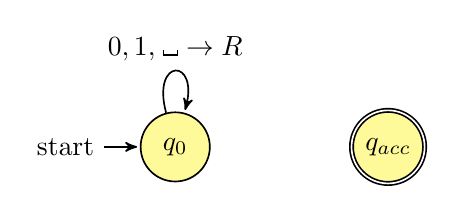
\begin{tikzpicture}[->,>=stealth',shorten >=1pt, auto, node distance=2cm, semithick]
      \tikzstyle{every state}=[text=black, fill=yellow!40]
      \node[initial,state] (q0)                    {$q_0$};
      \node[state,accepting] (qacc) [right of = q0, xshift = 20]{$q_{acc}$};
      \path (q0) edge  [loop above] node {$0, 1, \scalebox{1.5}{\textvisiblespace} \to R$} (q0)
     ;
    \end{tikzpicture}}
    \rangle$ 
    . This image string is not in $EQ_{TM}$ when $L(M'_x) \neq \emptyset$.
    
We will build $M'_x$ so that 
    $L(M'_{x}) = \Sigma^*$ when $M$ halts on $w$ and $L(M'_x) = \emptyset$ when $M$ loops on $w$.


Thus: when $\langle M,w \rangle \in HALT_{TM}$ it gets mapped to a string not in $EQ_{TM}$ and 
when $\langle M,w \rangle \notin HALT_{TM}$ it gets mapped to a string that is in $EQ_{TM}$.

\vfill

Define

\vspace{-15pt}

\begin{quote}
$F_1 =  ``$ On input $x$,
\begin{itemize}
\item[1.] Type-check whether  $x = \langle M, w \rangle$ for some TM $M$ and string $w$. 
If so, move to step 2; if  not, output  $\langle \hspace{2in} \rangle$
\item[2.] Construct the following machine $M'_x$:
\vspace{50pt}
\item[3.] Output $\langle M'_{x},
\scalebox{0.5}{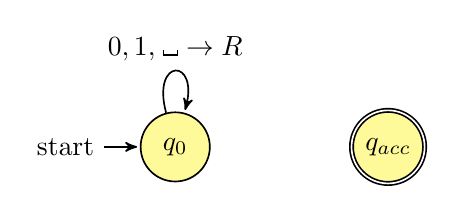
\begin{tikzpicture}[->,>=stealth',shorten >=1pt, auto, node distance=2cm, semithick]
      \tikzstyle{every state}=[text=black, fill=yellow!40]
      \node[initial,state] (q0)                    {$q_0$};
      \node[state,accepting] (qacc) [right of = q0, xshift = 20]{$q_{acc}$};
      \path (q0) edge  [loop above] node {$0, 1, \scalebox{1.5}{\textvisiblespace} \to R$} (q0)
     ;
    \end{tikzpicture}}
    \rangle$ "
\end{itemize}
\end{quote}

\vfill

Verifying correctness: (1) Is function well-defined and computable? (2) Does it have the 
translation property $x \in HALT_{TM}$ iff its image is {\bf not} in $EQ_{TM}$ ? 
\begin{center}
\begin{tabular}{|c|c|}
\hline
Input string &  Output string \\
\hline
$\langle M, w \rangle$ where  $M$ halts on $w$ & \phantom{\hspace{4in}} \\
& \\
& \\
& \\
$\langle M, w \rangle$ where $M$ loops on $w$ & \\
& \\
&\\ & \\
$x$ not encoding any pair of  TM and string   &  \\
& \\
& \\
\hline
\end{tabular}
\end{center}


\vfill

Conclude: $HALT_{TM} \leq_m \overline{EQ_{TM}}$
\newpage

\newpage 
Need computable function  $F_2: \Sigma^* \to \Sigma^*$  such that  $x \in HALT_{TM}$ iff 
$F_2(x)  \in  EQ_{TM}$.



{\it Strategy}:

\vspace{-15pt}

Map strings $\langle M, w \rangle$ to strings $\langle M'_{x},
\scalebox{0.5}{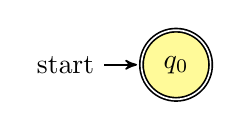
\begin{tikzpicture}[->,>=stealth',shorten >=1pt, auto, node distance=2cm, semithick]
      \tikzstyle{every state}=[text=black, fill=yellow!40]
      \node[initial,state,accepting] (q0)                    {$q_0$};
     ;
    \end{tikzpicture}}
    \rangle$ 
    . This image string is in $EQ_{TM}$ when $L(M'_x) = \Sigma^*$.
    
We will build $M'_x$ so that 
    $L(M'_{x}) = \Sigma^*$ when $M$ halts on $w$ and $L(M'_x) = \emptyset$ when $M$ loops on $w$.


Thus: when $\langle M,w \rangle \in HALT_{TM}$ it gets mapped to a string  in $EQ_{TM}$ and 
when $\langle M,w \rangle \notin HALT_{TM}$ it gets mapped to a string that is not in $EQ_{TM}$.

\vfill

Define

\vspace{-15pt}

\begin{quote}
$F_2 =  ``$ On input $x$,
\begin{itemize}
\item[1.] Type-check whether  $x = \langle M, w \rangle$ for some TM $M$ and string $w$. 
If so, move to step 2; if  not, output  $\langle \hspace{2in} \rangle$
\item[2.] Construct the following machine $M'_x$:
\vspace{50pt}
\item[3.] Output $\langle M'_{x},
\scalebox{0.5}{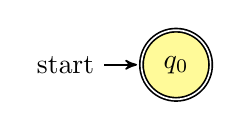
\begin{tikzpicture}[->,>=stealth',shorten >=1pt, auto, node distance=2cm, semithick]
      \tikzstyle{every state}=[text=black, fill=yellow!40]
      \node[initial,state,accepting] (q0)                    {$q_0$};
     ;
    \end{tikzpicture}}
    \rangle$ "
\end{itemize}
\end{quote}

\vfill

Verifying correctness: (1) Is function well-defined and computable? (2) Does it have the 
translation property $x \in HALT_{TM}$ iff its image is in $EQ_{TM}$ ? 
\begin{center}
\begin{tabular}{|c|c|}
\hline
Input string &  Output string \\
\hline
$\langle M, w \rangle$ where  $M$ halts on $w$ & \phantom{\hspace{4in}} \\
& \\
& \\
& \\
$\langle M, w \rangle$ where $M$ loops on $w$ & \\
& \\
&\\ & \\
$x$ not encoding any pair of  TM and string   &  \\
& \\
& \\
\hline
\end{tabular}
\end{center}


\vfill

Conclude: $HALT_{TM} \leq_m EQ_{TM}$
 

\newpage
\subsection*{Friday: Other models of computation}






Two models of computation are called {\bf equally expressive} when 
every language recognizable with the first model is recognizable with the second, and vice versa.

True / False: NFAs and PDAs are equally expressive.

True / False: Regular expressions and CFGs are equally expressive.


{\bf  Church-Turing Thesis} (Sipser p. 183): The informal notion of algorithm is formalized completely  and correctly by the 
formal definition of a  Turing machine. In other words: all reasonably expressive models of 
computation are equally expressive with the standard Turing machine.


\begin{center}
{\large \it  Some examples of models that are {\bf equally expressive} with deterministic Turing machines: }
\end{center}

\vfill

\fbox{ {\bf May-stay}  machines }
The May-stay machine model is the same as the usual Turing machine model,  except that
on each transition, the tape head may move L, move R, or Stay. 

Formally: $(Q, \Sigma, \Gamma, \delta, q_0, q_{accept}, q_{reject})$ where 
\[
  \delta: Q \times \Gamma \to Q \times \Gamma \times \{L, R, S\}
\]

{\bf Claim}: Turing machines and May-stay machines are equally expressive. {\it To prove \ldots}

To translate a standard TM to a may-stay machine: never use the direction $S$!


To translate one  of the  may-stay machines to standard TM:
any time TM would Stay, move right  then  left.

\begin{comment}
Formally: suppose $M_S =  (Q, \Sigma, \Gamma, \delta, q_0, q_{acc}, q_{rej})$
has $\delta: Q \times \Gamma \to Q \times \Gamma \times \{L, R, S\}$. Define
the Turing-machine
\[
  M_{new} =  (\phantom{\hspace{2.5in}})
\]

\vfill


\phantom{$M_{new}$ construction here \vspace{400pt}}
\vfill
\end{comment}

\vfill 

\fbox{ {\bf Multitape Turing machine}} A multitape Turing macihne with $k$ tapes
can be formally representated as 
$(Q, \Sigma,  \Gamma, \delta, q_0, q_{acc}, q_{rej})$ 
where $Q$ is the finite set of  states,
$\Sigma$ is the  input alphabet with  $\textvisiblespace \notin \Sigma$,
$\Gamma$  is the  tape alphabet with $\Sigma \subsetneq \Gamma$ ,
$\delta: Q\times \Gamma^k\to Q \times \Gamma^k \times \{L,R\}^k$ 
(where $k$ is  the number of  states)


If $M$ is a standard  TM, it is a $1$-tape machine.


To translate a $k$-tape machine  to  a standard TM:
Use a  new symbol to separate the contents of each tape
and keep track of location of  head with  special version of each
tape symbol. {\tiny Sipser Theorem 3.13} 

\includegraphics[width=2.5in]{resources/images/Figure314.png}

\newpage
\fbox{ {\bf Enumerators} } Enumerators give a different
model of computation where a language is {\bf produced, one string at a time},
rather than recognized by accepting (or not) individual strings.

Each enumerator machine has finite state control, unlimited work tape, and a printer. The computation proceeds
according to transition function; at any point machine may ``send'' a string to the printer.
\[
E  = (Q, \Sigma, \Gamma, \delta, q_0, q_{print})  
\]
$Q$ is the finite set of states, $\Sigma$ is  the output alphabet, $\Gamma$ is the 
tape alphabet ($\Sigma  \subsetneq\Gamma, 
\textvisiblespace \in \Gamma \setminus \Sigma$), 
\[
\delta:  Q  \times  \Gamma \times \Gamma \to  Q \times  \Gamma \times  \Gamma \times \{L, R\} \times  \{L, R\}
\]
where in state $q$, when the working tape is scanning character $x$ and the printer tape is scanning character $y$,
$\delta( (q,x,y) ) = (q', x', y', d_w, d_p)$ means transition to control state $q'$, write $x'$ on 
the working tape, write $y'$ on the printer tape, move in direction $d_w$ on the working tape, and move in direction 
$d_p$ on the printer tape. The computation starts in $q_0$ and each time the computation enters $q_{print}$
the string from the leftmost edge of the printer tape to the first blank cell is considered to be printed.

The language  {\bf  enumerated} by  $E$, $L(E)$, is $\{ w \in \Sigma^* \mid \text{$E$ eventually, at finite  time, 
prints $w$} \}$.

\begin{comment}
\begin{center}
\begin{tabular}{cc}
\includegraphics[width=3.5in]{Lec15enumerator.png}  & 
\begin{tabular}{|c|c|c|c|c|c|c|}
\hline
\multicolumn{1}{|c}{$q0$} &  \multicolumn{6}{c|}{\phantom{A}}\\
\hline
$\textvisiblespace ~*$& $\textvisiblespace$  & $\textvisiblespace$ & $\textvisiblespace$& $\textvisiblespace$& $\textvisiblespace$&  $\textvisiblespace$\\
\hline
$\textvisiblespace  ~*$& $\textvisiblespace$  & $\textvisiblespace$ & $\textvisiblespace$& $\textvisiblespace$& $\textvisiblespace$&  $\textvisiblespace$\\
\hline\hline
\multicolumn{7}{|c|}{\phantom{A}}\\
\hline
\phantom{AA} & \phantom{AA}& \phantom{AA}& \phantom{AA}& \phantom{AA}& \phantom{AA}& \phantom{AA} \\
\hline
\phantom{AA} & \phantom{AA}& \phantom{AA}& \phantom{AA}& \phantom{AA}& \phantom{AA}& \phantom{AA} \\
\hline
\hline
\multicolumn{7}{|c|}{\phantom{A}}\\
\hline
\phantom{AA} & \phantom{AA}& \phantom{AA}& \phantom{AA}& \phantom{AA}& \phantom{AA}& \phantom{AA} \\
\hline
\phantom{AA} & \phantom{AA}& \phantom{AA}& \phantom{AA}& \phantom{AA}& \phantom{AA}& \phantom{AA} \\
\hline
\hline
\multicolumn{7}{|c|}{\phantom{A}}\\
\hline
\phantom{AA} & \phantom{AA}& \phantom{AA}& \phantom{AA}& \phantom{AA}& \phantom{AA}& \phantom{AA} \\
\hline
\phantom{AA} & \phantom{AA}& \phantom{AA}& \phantom{AA}& \phantom{AA}& \phantom{AA}& \phantom{AA} \\
\hline
\hline
\multicolumn{7}{|c|}{\phantom{A}}\\
\hline
\phantom{AA} & \phantom{AA}& \phantom{AA}& \phantom{AA}& \phantom{AA}& \phantom{AA}& \phantom{AA} \\
\hline
\phantom{AA} & \phantom{AA}& \phantom{AA}& \phantom{AA}& \phantom{AA}& \phantom{AA}& \phantom{AA} \\
\hline
\end{tabular}
\end{tabular}
\end{center}


\newpage
\end{comment}

{\bf Theorem 3.21} A language is Turing-recognizable iff some enumerator enumerates it.

{\bf Proof, part 1}: Assume $L$ is enumerated by some enumerator, $E$, so $L = L(E)$. We'll use $E$ in a subroutine
within a high-level description of a new Turing machine that we will build to recognize $L$.

{\bf Goal}: build Turing machine $M_E$ with $L(M_E) = L(E)$.

Define $M_E$ as follows: $M_E = $ ``On input $w$,
\begin{enumerate}
\item Run $E$. For each string $x$ printed by $E$.
\item \qquad Check if $x = w$. If so, accept (and halt); otherwise, continue."
\end{enumerate}

{\bf Proof, part 2}: Assume $L$ is Turing-recognizable and there 
is a Turing  machine  $M$ with  $L = L(M)$. We'll use $M$ in a subroutine
within a high-level description of an enumerator that we will build to enumerate $L$.

{\bf Goal}: build enumerator $E_M$ with $L(E_M) = L(M)$.

{\bf Idea}: check each string in turn to see if it is in $L$.

{\it How?} Run computation of $M$ on each string.  {\it But}: need to be careful 
about computations that don't halt.

{\it Recall} String order for $\Sigma = \{0,1\}$: $s_1 = \varepsilon$, $s_2 = 0$, $s_3 = 1$, $s_4 = 00$, $s_5 = 01$, $s_6  = 10$, 
$s_7  =  11$, $s_8 = 000$, \ldots

Define $E_M$ as follows: $E_{M} = $ `` {\it ignore any input.} Repeat the following for $i=1, 2, 3, \ldots$
\begin{enumerate}
  \item Run the computations of $M$ on $s_1$, $s_2$, \ldots, $s_i$ for (at most) $i$ steps each
  \item For each of these $i$ computations that accept during the (at most) $i$ steps, print
  out the accepted string."
\end{enumerate}

\vfill

\fbox{ {\bf Nondeterministic Turing machine}}

At any point in the computation, the nondeterministic machine may proceed according to 
several possibilities: $(Q, \Sigma, \Gamma, \delta, q_0, q_{acc}, q_{rej})$ where 
\[
\delta: Q \times \Gamma \to \mathcal{P}(Q \times \Gamma \times \{L, R\})  
\]
The computation of a nondeterministic Turing machine is a tree with branching
when the next step of the computation has multiple possibilities. A nondeterministic
Turing machine accepts a string exactly when some branch of the computation tree 
enters the accept state.

Given a nondeterministic machine, we can use a $3$-tape Turing machine to 
simulate it by doing a breadth-first search of computation tree: one tape 
is ``read-only'' input tape, one tape simulates the tape of the nondeterministic
computation, and one tape tracks nondeterministic branching. {\tiny Sipser page 178} 

\vfill

{\bf Summary}

Two models of computation are called {\bf equally expressive} when 
every language recognizable with the first model is recognizable with the second, and vice versa.

To prove the existence of a Turing machine that decides / recognizes some language, 
it's enough to construct an example using any of the equally expressive models.

But: some of the {\bf performance} properties of these models are not equivalent.

\vfill 
\newpage

\subsection*{Week 9 at a glance}

\subsubsection*{Textbook reading: Section 5.3, 5.1, 3.2}

{\it For Monday}: Example 5.26 (page 237)

{\it For Wednesday}: Theorem 5.30 (page 238)

{\it For Friday}: Skim Section 3.2

{\it For Monday of Week 10}: Definition 7.1 (page 276)

\subsubsection*{Make sure you can:}
\begin{itemize}
\item Classify the computational complexity of a set of strings by determining whether it is decidable or undecidable and recognizable or unrecognizable.
\begin{itemize}
   \item State, prove, and use theorems relating decidability, recognizability, and co-recognizability.
   \item Prove that a language is decidable or recognizable by defining and analyzing a Turing machines with appropriate properties.
   \item Define and explain core examples of computational problems, including $A$**, $E$**, $EQ$**, (for ** either DFA or TM) and $HALT_{TM}$
\end{itemize}
\item Use diagonalization to prove that there are 'hard' languages relative to certain models of computation.
\item Use mapping reduction to deduce the complexity of a language by comparing to the complexity of another.
   \begin{itemize}
      \item Explain what it means for one problem to reduce to another
      \item Define computable functions, and use them to give mapping reductions between computational problems
      \item Define and explain $A_{TM}$ and $HALT_{TM}$
      \item Build and analyze mapping reductions between computational problems
      \item Distinguish between computability and complexity
      \item Articulate motivating questions of complexity
      \item Use appropriate reduction (e.g. mapping, Turing, polynomial-time) to deduce the complexity of a language by comparing to the complexity of another.
   \end{itemize}
\item  Describe several variants of Turing machines and informally explain why they are equally expressive.
   \begin{itemize}
   \item Define an enumerator
   \item Describe the language enumerated by an enumerator
   \item Use high-level descriptions to define and trace machines (Turing machines and enumerators)
   \item Apply dovetailing in high-level definitions of machines
   \item Define nondeterministic Turing machines
   \item State and use the Church-Turing thesis
   \end{itemize}
\end{itemize}


\subsubsection*{TODO:}
\begin{list}
   {\itemsep2pt}
   \item Student Evaluations of Teaching forms: Evaluations are open for completion anytime BEFORE 8AM on Saturday, March 16.
   Access your SETs from the Evaluations site
   \begin{quote}
        \url{https://academicaffairs.ucsd.edu/Modules/Evals}
   \end{quote}
   You will separately evaluate each of your listed instructors for each enrolled course. 

   **NEW** WINTER 2024 SET INCENTIVE LOTTERY: In Winter 2024, students who complete all of their student 
   evaluation forms for their undergraduate course will be entered into a lottery to win one of 
   5 \$100 Visa gift cards! To be entered into the lottery, students must complete at 
   least one instructor evaluation for EACH of their undergraduate courses. 
   They will be automatically entered when they have completed an instructor evaluation for 
   all of their undergraduate courses.

   \item Review quizzes based on class material each day.
   \item Test this Friday in Discussion section.
   \item Homework assignment 5 due next Thursday.
\end{list}

\end{document}
